%!TEX root = main.tex
%=================TD functions==================
\def\boldcommandlist{\@elt OP,\@elt OPs,}
\def\@elt#1,{%
 \expandafter\def\csname#1\endcsname{\textbf{#1}\xspace}
}
\boldcommandlist

\def\topColorList{\@elt TOP,\@elt TOPs,}
\def\@elt#1,{%
 \expandafter\def\csname#1\endcsname{\textcolor{TOP}{\textbf{#1}}\xspace}
}
\topColorList

\def\chopColorList{\@elt CHOP,\@elt CHOPs,}
\def\@elt#1,{%
 \expandafter\def\csname#1\endcsname{\textcolor{CHOP}{\textbf{#1}}\xspace}
}
\chopColorList

\def\sopColorList{\@elt SOP,\@elt SOPs,}
\def\@elt#1,{%
 \expandafter\def\csname#1\endcsname{\textcolor{SOP}{\textbf{#1}}\xspace}
}
\sopColorList

\def\datColorList{\@elt DAT,\@elt DATs,}
\def\@elt#1,{%
 \expandafter\def\csname#1\endcsname{\textcolor{DAT}{\textbf{#1}}\xspace}
}
\datColorList

\def\matColorList{\@elt MAT,\@elt MATs,}
\def\@elt#1,{%
 \expandafter\def\csname#1\endcsname{\textcolor{MAT}{\textbf{#1}}\xspace}
}
\matColorList


\def\compColorList{\@elt COMP,\@elt COMPs,}
\def\@elt#1,{%
 \expandafter\def\csname#1\endcsname{\textcolor{COMP}{\textbf{#1}}\xspace}
}
\compColorList

\def\redcommandlist{\@elt missingImage,}
\def\@elt#1,{%
 \expandafter\def\csname#1\endcsname{\textcolor{red}{\textbf{#1}}\xspace}
}
\redcommandlist




%===============================================

\chapter{Lecture 1, Introduction and 2D-Processing}
\label{chap:Introduction}
\section{Notes}
\color{textStd}

\begin{center}
\begin{figure}[h!]
\tikzset{concept/.append style={fill={none}}}
\begin{tikzpicture}
  \path[mindmap,concept color=textStd,text=textStd]
    node[concept] {Introduction}
    [clockwise from=0]
    child[concept color=CHOP] {
      node[concept] {CHOPs}
      % }
      [clockwise from=90]
      child { node[concept] {Exporting} }
      child { node[concept] {Audio} }
      child { node[concept] {Trail CHOP} }
      % child { node[concept] {TOPs} }
      % child { node[concept] {pro\-gramming languages} }
      % child { node[concept] {software engineer\-ing} }
    }
    child[concept color=TOP] {
      node[concept] (fm) {TOPs}
      [clockwise from=-30]
    }
    child[concept color=blue] { node[concept] (pm){GUI}
        [clockwise from=180] child[concept]{node[concept] {Navigation and COMPS}}
        }
    child[concept color=red] { node[concept] (si) {Student's interests} }
    child[concept color=orange] { node[concept] (op) {Output}
        [clockwise from=180] child[concept]{node[concept]{Window COMP
        }}
        child[concept]{node[concept]{Movie Out
        }}
    };


% \begin{pgfonlayer}{background}
%     \draw [circle connection bar]
%       (fm) edge (sd)
%       (fm) edge (pm);
%   \end{pgfonlayer}

\end{tikzpicture}
\caption{Lecture Contents}
\end{figure}
\end{center}

% \begin{figure}[H]
% 	\begin{center}
% 		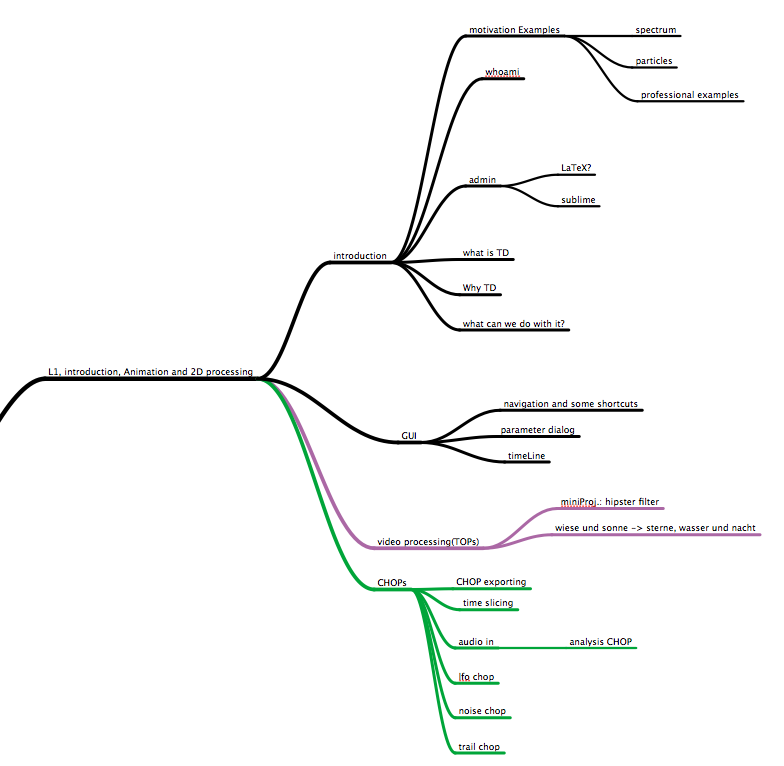
\includegraphics[width = 18cm]{img/lecture1.png}
% 		\caption{overview}
% 		\label{fig:overview}
% 	\end{center}
% \end{figure}

\section{About}

About me:
\link{http://www.vimeo.com/titled}{my vimeo site}
% \href


TouchDesigner is coming from sideFX/Houdini. Now made by the company \textit{derivative} \\

Other products, more or less similar to TD:
\begin{itemize}
	\item vvvv
	\item quarz composer
	\item Max/MSP/Jitter
	\item processing
	\item also game engines(Unity, Unreal, ...)
\end{itemize}

What can we do with TD?
\begin{itemize}
	\item \link{https://www.derivative.ca/Events/2014/Gravity/}{gravity}
	\item \link{https://vimeo.com/55818038}{v squares Mapping Reel}
	\item \link{https://vimeo.com/groups/touchdesigner/videos/71991897}{NiN tour}
\end{itemize}


% projects in this lecture:
% \begin{itemize}
% 	\item hipster filter
% 	\item video playback (mention ffmpeg, hap encoding)
% 	\item sunRise -> water, stars, night
% 	\item fist rendering
% 	\item noise ball
% 	\item off-line rendering
% \end{itemize}
% subsection subsection_name (end)

\section{Getting Help}
\begin{itemize}
	\item Here (in the future hopefully)
	\item The Book \link{http://www.amazon.com/Multimedia-Programming-using-Max-TouchDesigner/dp/1849699712}{Multimedia Programming using Max/MSP and TouchDesigner}
	\item The open source book \link{http://book.nvoid.com/}{introduction to TouchDesigner}
	\item \link{http://www.derivative.ca/wiki088/index.php?title=Main\_Page}{the TD Wiki}
	\item the TouchDesigner OP Snippets. A useful collection of examples for each operator, accessible via TouchDesigner's help menu.
	\item \link{http://www.derivative.ca/Forum/}{The TD Forums}
	\item \link{https://www.facebook.com/groups/touchdesignerhelp/}{the TouchDesigner Help Group on Facebook}
\end{itemize}

\section{The User Interface} % (fold)
\label{sub:the_user_interface}

In figure \ref{fig:ui} we can see the graphical user interface of TD. Two good videos explaining the first steps(like navigating in the UI etc.) are:
\begin{itemize}
	\item \link{https://vimeo.com/10056323}{Part A}
	\item \link{https://vimeo.com/10106354}{Part B}
\end{itemize}

\begin{figure}[H]
	\begin{center}
		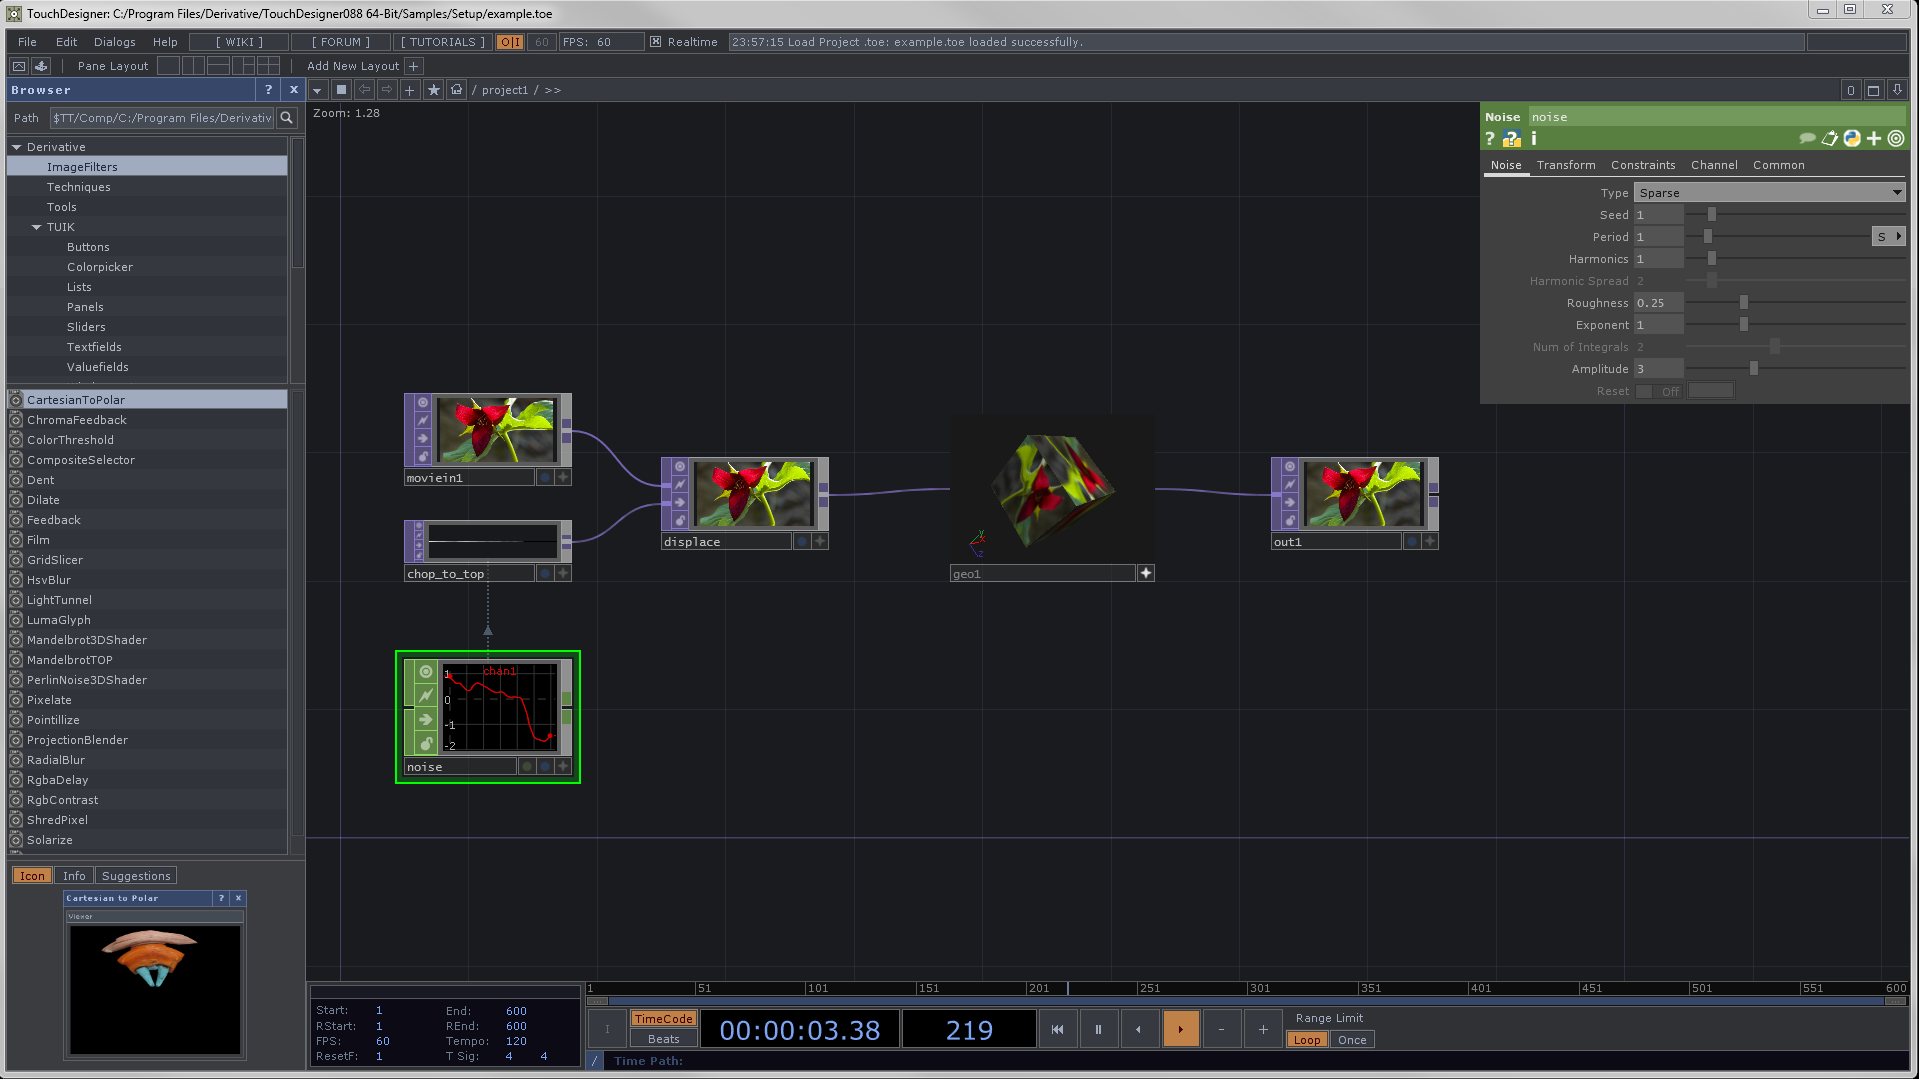
\includegraphics[width = 14cm]{img/gui.png}
		\caption{The User Interface}
		\label{fig:ui}
	\end{center}
\end{figure}

To the left, there is the \textbf{Palette Browser} \index{Palette Browser}, which holds reusable code, \COMPs, made by us or the factory. The big area in the center is called a \textbf{pane} \index{Pane}. Here we can see our \textbf{network}, consisting of operators, or \OPs for short.\\
To the upper right, we have the \textbf{Parameter Dialog}, see also fig. \ref{fig:parDialog},which holds all the options for a currently selected \OP\footnote{In TD we can select multiple \OPs using box selection or the shift key. When we select similar \OPs we can adjust all their values at once in the parameter dialog }.\\

\begin{figure}[H]
	\begin{center}
		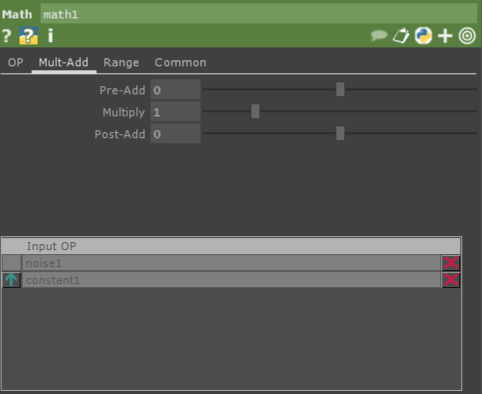
\includegraphics[width = 10cm]{img/parameterDialog.png}
		\caption{the Parameter Dialog}
		\label{fig:parDialog}
	\end{center}
\end{figure}

We can add \OPs by pressing \keystroke{tab} or double clicking in an empty area of the network, to bring up the \textbf{OP Create Dialog}, as depicted in fig. \ref{fig:opCreate}. \\

\begin{figure}[H]
	\begin{center}
		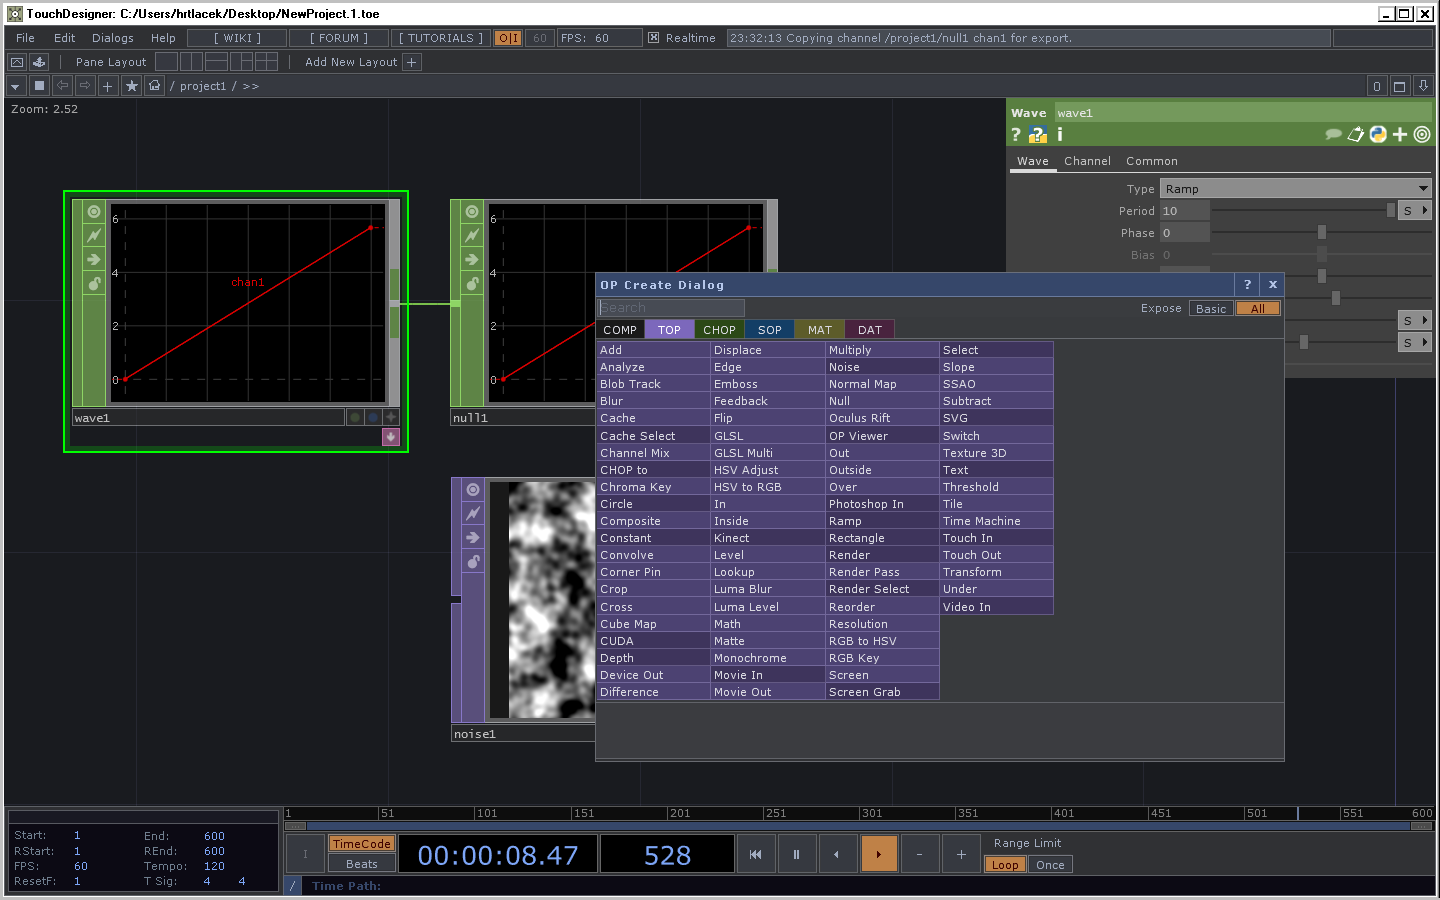
\includegraphics[width = 14cm]{img/opCreate.png}
		\caption{The OP create Dialog}
		\label{fig:opCreate}
	\end{center}
\end{figure}



We can connect \OPs by clicking at outputs and inputs of \OPs. We can only connect \OPs that are in the same \textit{family}, so \TOPs with \TOPs and \CHOPs with \CHOPs\footnote{There are ways to convert between families though, and \COMPs can have inputs whose family we can define}. We can disconnect \OPs by right-clicking at the cord and choosing \verb|disconnect| or by clicking at the inlet of the connected \OP and dragging away to an empty area.
\begin{framed}
	If we look closely at the OP Create Dialog, we can see that some of the \OPs are colored more dark and others are more light. The darker ones are \textit{generators}, so they produce data, the lighter ones are called \textit{filters} so they process data, and need input.

\end{framed}

Let's have a quick look at the header of the parameter dialog: The header section in the parameter dialog displays the type and name of the operator and provides a number of buttons for basic operations as described below. The background color of the parameter header indicates the operator's family type.

\begin{figure}[H]
	\begin{center}
		
\includegraphics[width = 14cm]{img/ParameterHeader.png}
		\caption{Parameter Dialog Header}
		\label{fig:parHeader}
	\end{center}
\end{figure}




Top Section
\begin{itemize}
	\item OP Type (Geometry \COMP in this case)
	\item OP Name
\end{itemize}

Bottom Section
\begin{itemize}
	\item Operator Help
	\item Python Class Help
	\item Operator Info
	\item Comment
	\item Clipboard
	\item Python/Tscript Operator Language Toggle
	\item Hide/Show Default Parameters
\end{itemize}

The most important ones for us at the moment are the Operator Help, the Operator Info and the Show default Parameters buttons: \\
The operator info shows us important information about the data the Operator holds (such as resolution for \TOPs or number of vertices for \SOPs) but also displays errors if we messed up something.\\
\begin{framed}
	Usually we access the Operator info just by middle-mouse clicking on the \OP itself, instead of clicking on the operator info button. That way you always have all the info always at your fingertips.
\end{framed}

\begin{figure}[H]
	\centering
	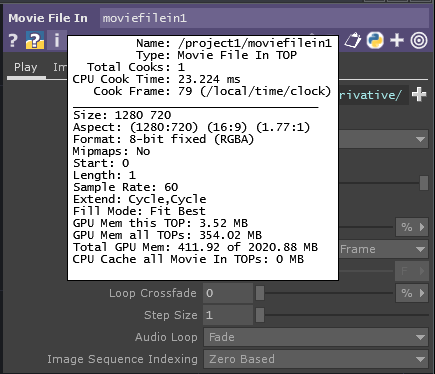
\includegraphics[width=10cm]{img/info.PNG}
	\caption[shortCaption]
	{CAPTION MISSING}
	\label{fig:label}
\end{figure}








\section{The Operator Families}
\subsection{CHOPs} % (fold)
\label{sub:CHOPs}

\begin{figure}[H]
	\begin{center}
		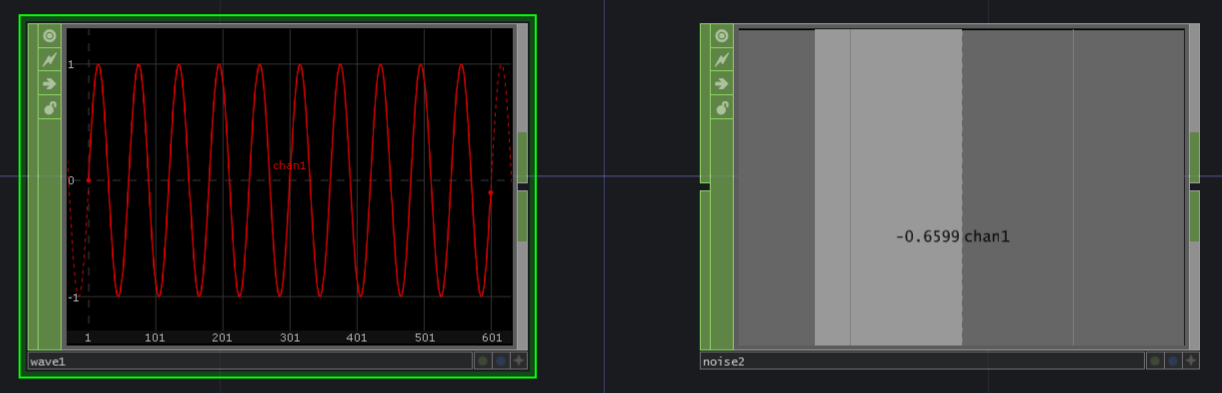
\includegraphics[width = 14cm]{img/chops.png}
		\caption{chops}
		\label{fig:chops}
	\end{center}
\end{figure}

\CHOPs are Channel Operators. Generally speaking, we could say, \CHOPs are there for movement, animation, control of parameters, control signals and streaming numeric data. For example an audio file could be loaded using the Audio File In \CHOP, an LFO\footnote{Low-Frequency Oscillator} can be created with an LFO \CHOP.  \CHOPs can contain any number of samples, and any number of channels. Also there are \CHOPs for OSC in/output, Audio in/output, MIDI, DMX, Kinect, Leap Motion and many other interfaces.

\subsection{TOPs} % (fold)
\label{sub:TOPs}

\begin{figure}[H]
	\begin{center}
		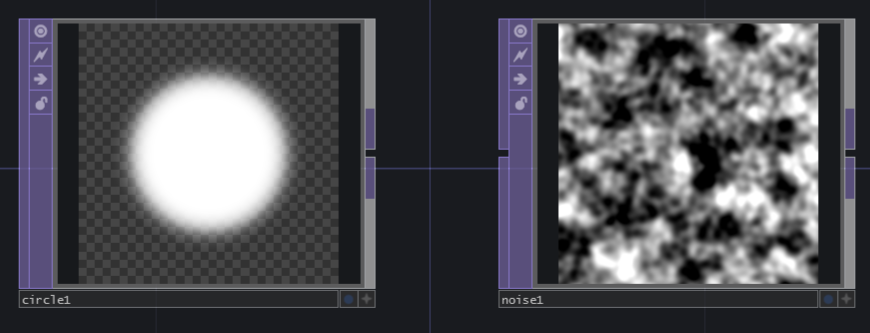
\includegraphics[width = 14cm]{img/tops.png}
		\caption{tops}
		\label{fig:tops}
	\end{center}
\end{figure}
\TOPs are Texture Operators. They hold image data, or other data in 2 dimensional/Image form. We find effects for image processing in this category. All of the Texture Operators are GPU accelerated, and therefore can be very efficient. Don't forget that images are just data, if we want to use \TOPs for working on other data than images, that's fine too, just the format has to be right. We will talk about moving between OP Families later.


\subsection{COMPs} % (fold)
\label{sub:COMPs}


\begin{figure}[H]
	\begin{center}
		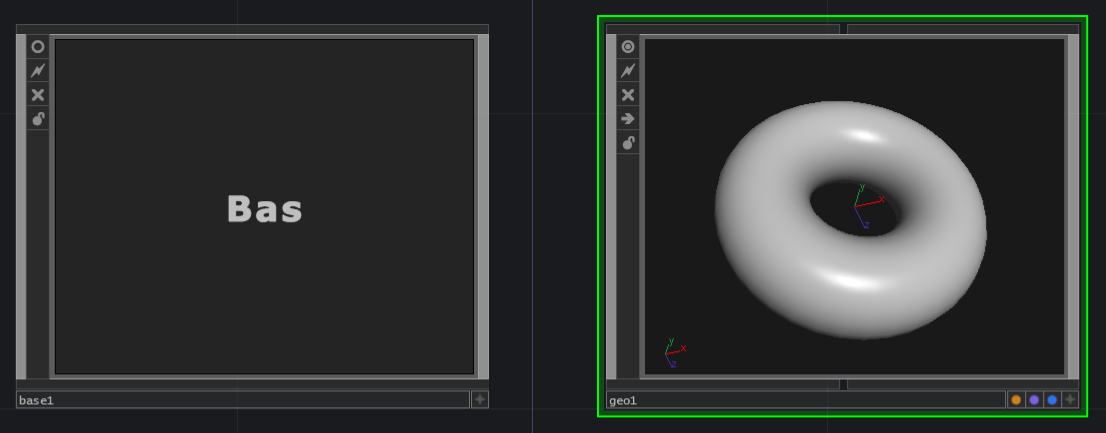
\includegraphics[width = 14cm]{img/comps.png}
		\caption{comps}
		\label{fig:comps}
	\end{center}
\end{figure}
Components, or \COMPs for short. If you come from Max/MSP or pd you can think of them as subpatchers. But in TD there are many different kinds of subpatchers.\\
\COMPs can contain other \OPs. They allow us to build up hierarchies and to organize our networks in a more tidy way. But also, there are specialized \COMPs for different purposes. If we just want to pack a network into some kind of  self-contained box we should always use a Base \COMP \index{Base Comp}. If we want our result to have a GUI also, we should rather use a Container \COMP \index{Container Comp}. Later, in chapter \ref{chap:3D_intro} we will see specialized \COMPs for 3D rendering such as a Geometry \COMP.


\subsection{SOPs} % (fold)
\label{sub:sops}

\begin{figure}[H]
	\begin{center}
		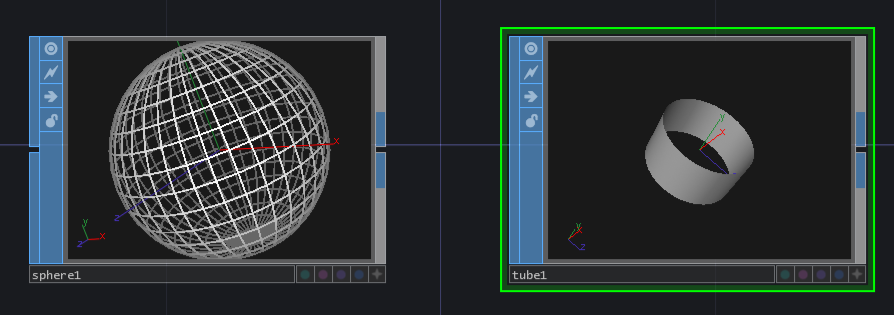
\includegraphics[width = 14cm]{img/sops.png}
		\caption{sops}
		\label{fig:sops}
	\end{center}
\end{figure}

\SOPs stands for Surface Operators. They are operators acting in 3d space. They let us model in a procedural way, transform, scale, extrude, twist and edit geometry procedurally. SOPs are processed on the CPU and then sent to a render TOP to be rendered to an image. Their CPU consumption heavily depends on the number of point they are dealing with. Also SOPs can contain different types of data: Polygons, NURBS, Meshes, primitives, bezier.

\subsection{MATs} % (fold)
\label{sub:mats}

\begin{figure}[H]
	\begin{center}
		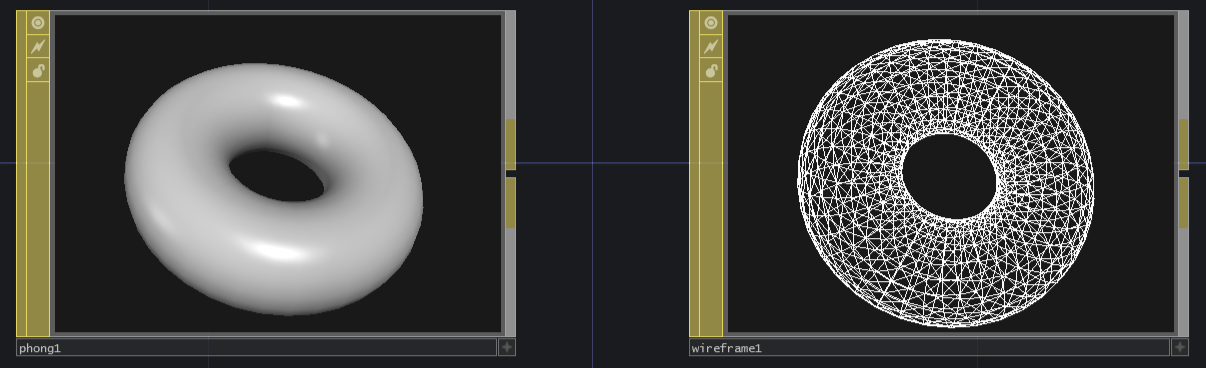
\includegraphics[width = 14cm]{img/mats.png}
		\caption{MATs}
		\label{fig:mats}
	\end{center}
\end{figure}
\MATs or Materials are used to shade geometry, so, this determines the look of our 3d objects. We are going to visit them later.

\subsection{DATs} % (fold)
\label{sub:dats}


\begin{figure}[H]
	\begin{center}
		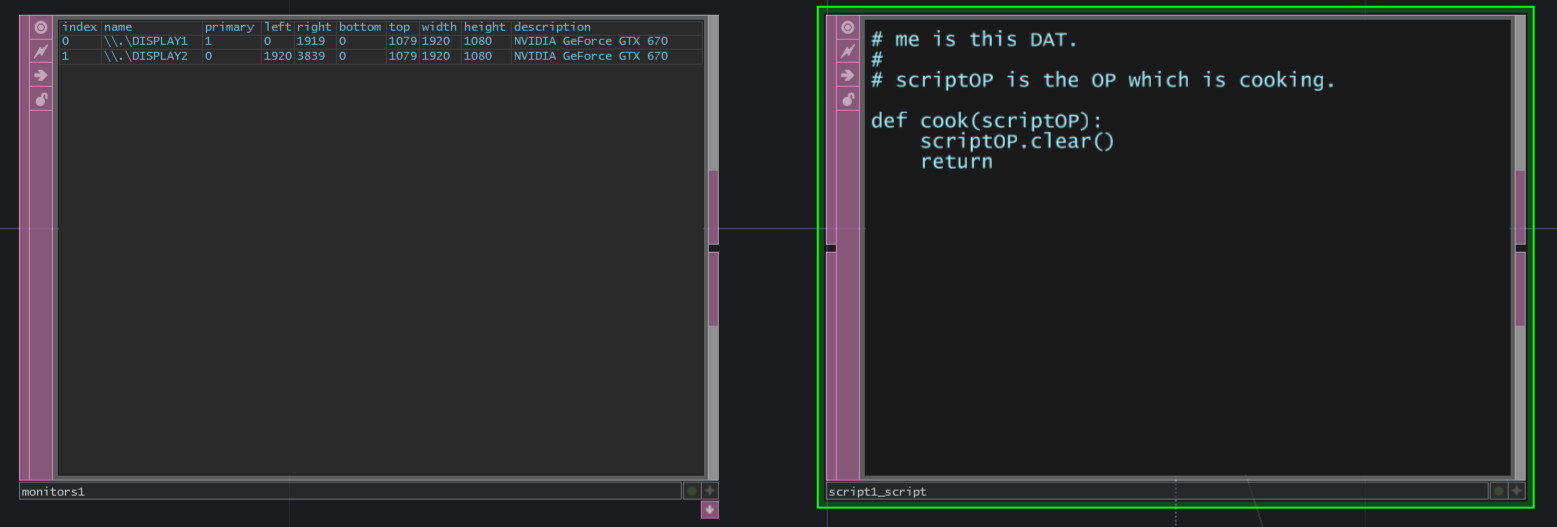
\includegraphics[width = 14cm]{img/dats.png}
		\caption{DATs}
		\label{fig:dats}
	\end{center}
\end{figure}

\DATs or Data operators, let us enter, edit and process text, code, tables and they handle incoming data as OSC, UDP, TCP/IP, MIDI etc. as well as output data using these protocols/interfaces.

\section{TOPs Introduction}

\subsection{Simple 2D Generation and Processing}

\subsubsection{Effects on Web-Cam input}
For a first simple example, let's consider \ref{fig:simple2d}. The idea is just that we take our webcam (or other video input device) and apply some effects to that stream of images.\\
As an exercise, look at the block diagram and implement it yourself in TD. The names of the Operators are identical to the labels, and remember you already know what OP family is the one for image processing, so make sure you're looking under \TOPs. Don't forget to play around with the parameters of each \OP!



  \begin{figure}[htb]
  \centering


  % \resizebox{10cm}{!}{%
  \begin{tikzpicture}[auto, thick, node distance=2.3cm, >=triangle 45]

  \draw node at (5,0) [block] (inp) {\Large$Video\ Device\ In $};
  \draw node [block, right of=inp, node distance = 4cm] (blur) {\Large$Blur$};
  \draw node [block, right of=blur, node distance = 3cm] (transform) {\Large$Transform$};
	\draw node [block, right of=transform, node distance = 3cm] (level) {\Large$Level$};
  % \draw node right of (inp) (blur) {$blur$}
  % \draw node at (5,-3) [block] (del2) {\Large$\ \ \ \ \ \ \ \ z^{-m}\ \ \ \ \ \ \ \ $};
  % \draw node at (0, -1.5) [mult] (m1) {\Large$-1$};
  % \draw node at (10, -1.5) [mult] (m2) {\Large$-1$};

  \draw[->] (inp) -- node {}(blur);
  \draw[->] (blur) -- node {}(transform);
  \draw[->] (transform) -- node {}(level);
  % \draw[->] (m2) |- node {}(del2);
  % \draw[->] (del2) -| node {}(m1);
  % \draw[->] (m1) |- node {}(del1);

  \end{tikzpicture}
  \caption{Basic real-time image processing Example.}
  \label{fig:simple2d}
\end{figure}



\begin{figure}[H]
	\begin{center}
		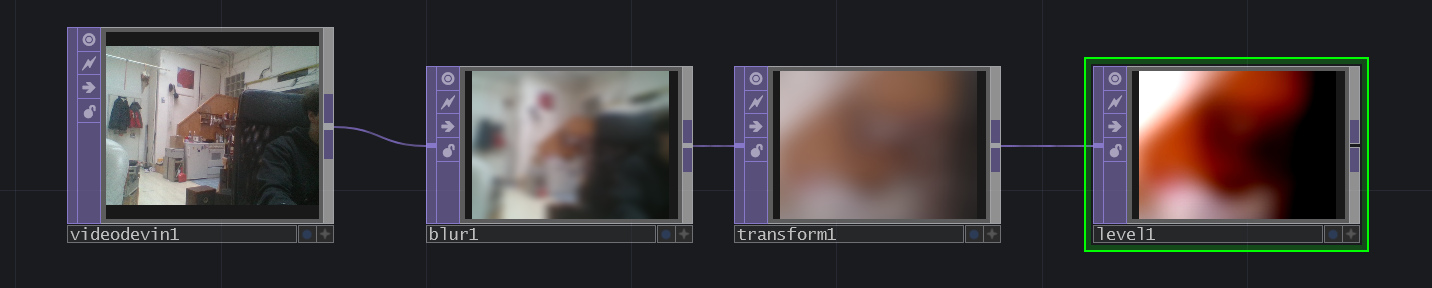
\includegraphics[width = 10cm]{img/simple2Dproc.PNG}
		\caption{The TD network representing the block diagram above.}
		\label{fig:simpleProcTD}
	\end{center}
\end{figure}


\subsubsection{Cooking and Resolution Inheritance}
Before moving on to more spectacular results such as moving images and 3D scenes, let's make sure we throughly understand how TD manages resolutions. TD in general wants to help us and wants to make clever decisions about optimization. So it will make decisions about resolutions and when it is necessary to \textbf{cook} an \OP \index{cooking}.
\begin{framed}
	The Term 'cooking' in TD refers to processing. This is not specific to \TOPs. If an \OP cooks it means it does work, consumes CPU/GPU resources and produces output data. If it does not 'cook' it just outputs static data or no data and does not consume resources (except of memory). If you look at the cords connecting the \OPs in our last example, you should see a slight animation, indicating that data is indeed flowing (because our web cam continuously delivers frames to process.) In our next example, this won't be the case.
\end{framed}
To explore resolution management, let's build a little network that produces a nice graphic with some simple shapes and some compositing. What we plan to do is depicted in Figure \ref{fig:graphicalbd}.


  \begin{figure}[H]
  \centering


  % \resizebox{10cm}{!}{%
  \begin{tikzpicture}[auto, thick, node distance=2.3cm, >=triangle 45]

  \draw node at (5,0) [block] (circle) {\Large$Circle $};
  \draw node [block, below of=circle, node distance = 2cm] (rectangle) {\Large$Rectangle$};
  \draw node [block, below of=rectangle, node distance = 2cm] (constant) {\Large$Constant$};

	\draw node [block, right of=circle, node distance = 3cm] (XOR) {\Large$XOR$};
	\draw node [block, right of=XOR, node distance = 3cm] (XOR2) {\Large$XOR$};
	\draw node [block, right of=XOR2, node distance = 3cm] (over) {\Large$over$};
	\draw node [block, below of=over, node distance = 3cm] (constant2) {\Large$constant$};

  % \draw node right of (inp) (blur) {$blur$}
  % \draw node at (5,-3) [block] (del2) {\Large$\ \ \ \ \ \ \ \ z^{-m}\ \ \ \ \ \ \ \ $};
  % \draw node at (0, -1.5) [mult] (m1) {\Large$-1$};
  % \draw node at (10, -1.5) [mult] (m2) {\Large$-1$};

  \draw[->] (circle) -- node {}(XOR);
  \draw[->] (rectangle) -| node {}(XOR);
  \draw[->] (XOR) -- node {}(XOR2);
  \draw[->] (constant) -| node {}(XOR2);
  \draw[->] (XOR2) -- node {}(over);

\draw[->] (constant2) -- node {}(over);

  % \draw[->] (m2) |- node {}(del2);
  % \draw[->] (del2) -| node {}(m1);
  % \draw[->] (m1) |- node {}(del1);

  \end{tikzpicture}
  \caption{Network for producing a simple geometric graphic}
  \label{fig:graphicalbd}
\end{figure}

Give it a try before looking at the screen-shot in figure \ref{fig:graphical}. The Blocks labeled $XOR$ are just \link{http://derivative.ca/wiki099/index.php?title=Composite\_TOP}{Composite} \TOPs, whose mode has been switched to the XOR operation\footnote{XOR stands for exclusive OR, a common boolean operation that will be positive if and only if \textbf{one} of the two inputs is positive. It will also be False/not positive if both of the inputs are True/Positive.}.\\
Play around with the parameters a bit, I adjusted the scale and position parameters of both the circle and the rectangle, and used the rotate parameter of the rectangle to arrive at what's depicted in Figure \ref{fig:graphical}.\\
Now let's look at the resolutions we are operating with. When you middle mouse click on the \OPs, you can see their resolutions. By default they are all at $256 \times 256$. Now that's a bit poor, so let's do something about this. All \OPs have a common page in their parameter dialog. It contains parameters common to that family of \OPs, hence the name. In figure \ref{fig:topCommon} you can see the common page of one of the \link{http://derivative.ca/wiki099/index.php?title=Composite\_TOP}{Composite} \TOPs.
\begin{figure}[H]
	\centering
	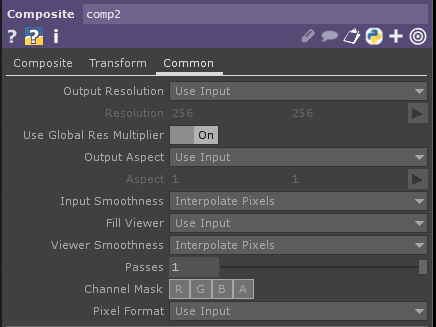
\includegraphics[width=10cm]{img/TOPcommonPars.PNG}
	\caption[TOP common parameters]
	{TOP common pars}
	\label{fig:topCommon}
\end{figure}


Since this \OP is a \glqq{}filter\grqq{}, so it has an input, it has the option to use its input to determine the output resolution. This will be default for all filter \OPs.\\
If you now go to the \refTOP{Circle}, you will find it has a resolution parameter that is set to $256 \times 256$. Try changing it to $1024\times1024$. You will see, if you zoom in a bit, the resolution is quite a bit better, for the circle at least.\\
The composite \OPs can take multiple input signals, so which resolution should they take?\\
By default, always the last \OP's resolution is used. So if you also change the resolution of the \refTOP{Rectangle}, the two \refTOP{Constant}s you will find the whole network is running at a higher resolution.



\begin{figure}[H]
	\centering
	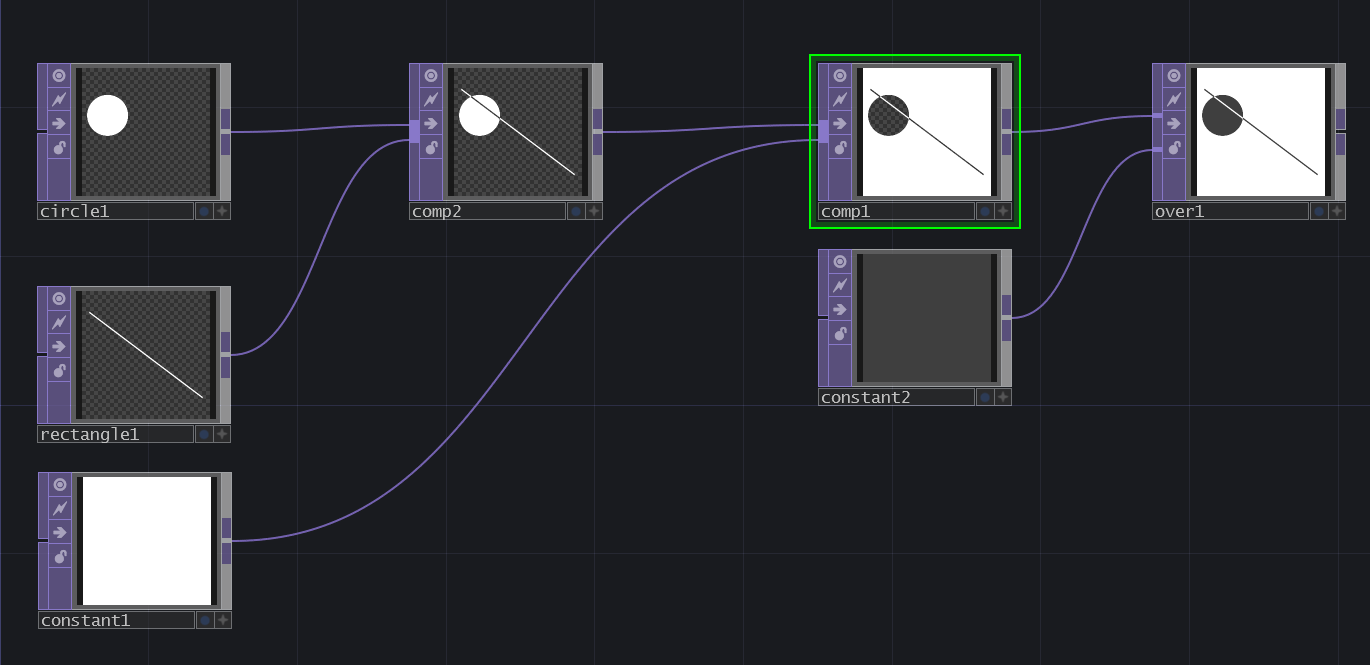
\includegraphics[width=\textwidth]{img/graphical.PNG}
	\caption[shortCaption]
	{CAPTION MISSING}
	\label{fig:graphical}
\end{figure}


\noindent\rule{12cm}{0.4pt}
\\
	\textbf{Exercise:}
	The last example was inspired by \link{http://derivative.ca/events/2018/BlokArtwork/}{this}. Try to imitate the other examples there!
\\
\noindent\rule{12cm}{0.4pt}



\subsubsection{TOP common page}

Looking at Figure \ref{fig:topCommon}, you can see a lot of parameters that rather seem technical, such as resolution and bit depth. Don't be fooled, some of these can be really interesting from an artistic/creative point of view. As an example we will explore the parameter \texttt{Channel Mask}. For a full description of all parameters, please look at the \link{http://www.derivative.ca/wiki099/index.php?title=TOP\_Generator\_Common\_Page}{TOP Generator Common Page Wiki entry} or the \link{http://www.derivative.ca/wiki099/index.php?title=TOP\_Filter\_Common\_Page}{TOP Filter Common Page Wiki entry}.\\
Let's put a \refTOP{Transform} after our current network. Use its parameters to move the whole image slightly to the right. After that, go to the \refTOP{Transform}'s Common Page and under \texttt{Channel Mask}, switch off the button with the Label 'R'. This deactivates the \TOP's effect for the red channel. The result is a commonly used effect:

\begin{figure}[H]
	\centering
	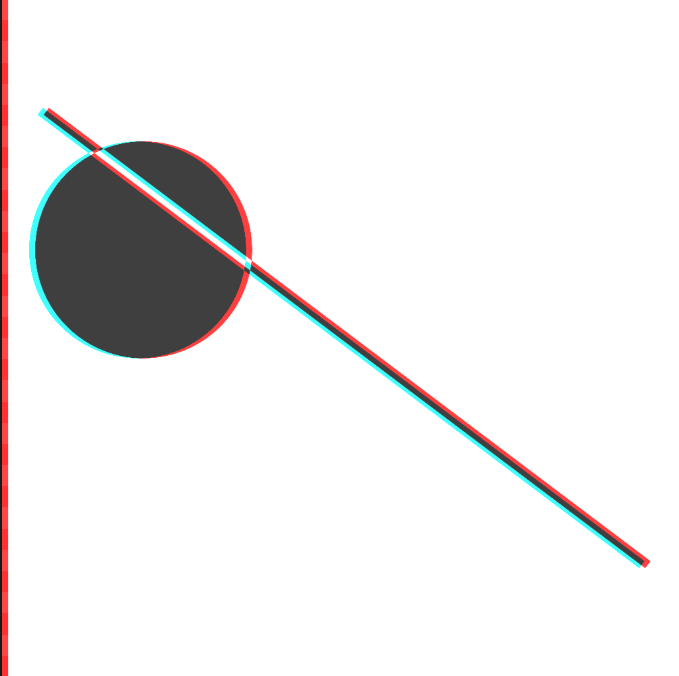
\includegraphics[width=7cm]{img/R_shift.PNG}
	\caption[All but the red channel Shifted]
	{All but the red channel Shifted}
	\label{fig:label}
\end{figure}


\subsection{Simple Output}
So we did process some live input and observed the results by just looking at the \OPs viewers. But in reality, we need some kind of output, be it saving an image or video to disk, be it full-screen output to one or more projectors, LED walls, or maybe we output DMX to control lights.\\
As you can see, different situations demand different output techniques, but mainly to keep us motivated, let's just record a quick movie and try out full-screen output to one monitor.\\

\subsubsection{Recording Movies and Images}

Let's keep thing simple for now. Use our previous example and put down a \refTOP{Movie\_File\_Out}. In its parameters, you can choose if you want to record an image or a movie, you can choose the location where the file will be saved and other parameters such as compression.\\
Just switch on record and switch it off again when you want to finish your recording.\\
TD allows us to also record 'offline' so it wont loose any frames and takes time to render frames. This is especially important if we built a network that exceeds the real-time performance of our machine. We will get into this topic at a later point of this document.

\subsubsection{Full-Screen Output}
\index{Window COMP}
For this topic, we will build a very simple new network, but finally one with some movement. When looking at the block diagram in Figure \ref{fig:outputDispl} beware that our block diagrams are slowly going to get more abstract and less explicit. For example there is no $Output$ \TOP\footnote{There is an Out \TOP, but it isn't meant here and we are going to see what it does soon.}. What's meant here is that this is going to be the output of our network, going to the screen. The network is supposed to load and play a movie file and distort it using the \refTOP{Displace}. This should then be output using a Window \COMP.

	\begin{figure}[H]
	\centering


	% \resizebox{10cm}{!}{%
	\begin{tikzpicture}[auto, thick, node distance=2.3cm, >=triangle 45]

	\draw node at (5,0) [block] (movie) {\Large$Movie\ File\ In $};
	\draw node [block, below of=movie, node distance = 2cm] (noise) {\Large$Noise$};
	\draw node [block, right of=movie, node distance = 5cm] (displace) {\Large$displace$};

	\draw node [block, right of=displace, node distance = 3cm] (output) {\Large$output$};
	% \draw node [block, right of=XOR, node distance = 3cm] (XOR2) {\Large$XOR$};
	% \draw node [block, right of=XOR2, node distance = 3cm] (over) {\Large$over$};
	% \draw node [block, below of=over, node distance = 3cm] (constant2) {\Large$constant$};

  % \draw node right of (inp) (blur) {$blur$}
  % \draw node at (5,-3) [block] (del2) {\Large$\ \ \ \ \ \ \ \ z^{-m}\ \ \ \ \ \ \ \ $};
  % \draw node at (0, -1.5) [mult] (m1) {\Large$-1$};
  % \draw node at (10, -1.5) [mult] (m2) {\Large$-1$};

  \draw[->] (movie) -- node {}(displace);
  \draw[->] (noise) -| node {}(displace);
  \draw[->] (displace) -- node {}(output);
%   \draw[->] (constant) -| node {}(XOR2);
%   \draw[->] (XOR2) -- node {}(over);

% \draw[->] (constant2) -- node {}(over);

  % \draw[->] (m2) |- node {}(del2);
  % \draw[->] (del2) -| node {}(m1);
  % \draw[->] (m1) |- node {}(del1);

  \end{tikzpicture}
  \caption{Network for producing a simple geometric graphic}
  \label{fig:outputDispl}
\end{figure}

Build up the network and maybe lower the Displace \TOP's \texttt{Displace Weight} parameter to about $0.06$ (both the x and the y value) to make the effect less extreme. Also switch off \texttt{Monochrome} of the \refTOP{Noise}.\\
Finally enter the following expression into the Noise \TOP's Translate z parameter as depicted in \ref{fig:expressionNoiseTOP}: \texttt{absTime.frame/100}.

\begin{framed}
	What does the expression \texttt{absTime.frame/100} mean? \texttt{absTime.frame} always returns the current absolute frame, so an integer that stands for the current frame number since we started TD. It is an ever increasing number.\\
	We can use that to translate the Noise. What does that mean? Noise is a collection of quasi-random values. These values are computed along a domain, and this domain can be shifted. Translate the noise \TOP's output in X or Y and you will immediately see that it just 'moves' the image left/right or up/down. Moving in Z moves in another dimension, seemingly creating a \textbf{continuous} set of new random values. Continuous means that the image does not 'jump', it gradually changes, which is often what we want.\\
	The division, so \texttt{/100} just slows down this behavior since that movement happens 100 times slower.
\end{framed}

\begin{figure}[H]
	\centering
	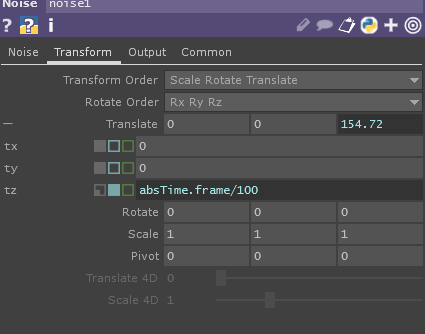
\includegraphics[width=10cm]{img/noiseTopExpr.PNG}
	\caption[An expression in the Transform parameter of the Noise \TOP.]
	{Expression in Noise TOP}
	\label{fig:expressionNoiseTOP}
\end{figure}



\begin{figure}[H]
	\centering
	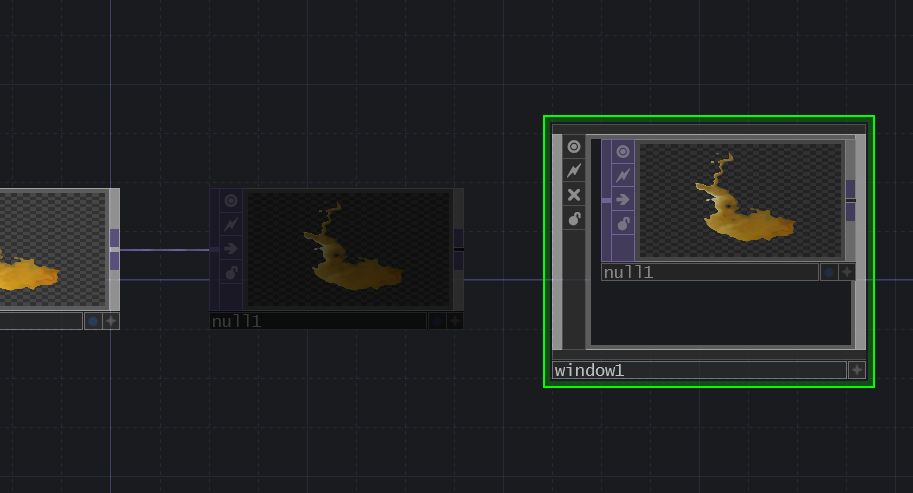
\includegraphics[width=\textwidth]{img/dragOnWindow.PNG}
	\caption[shortCaption]
	{CAPTION MISSING}
	\label{fig:label}
\end{figure}

\begin{figure}[H]
	\centering
	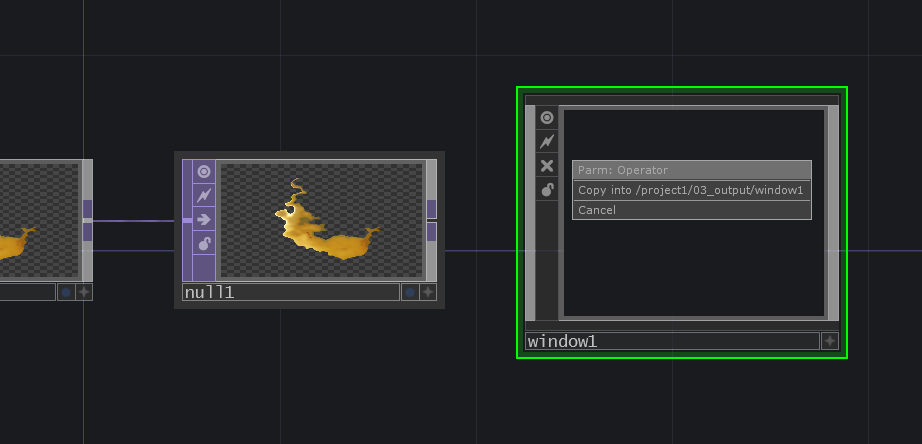
\includegraphics[width=\textwidth]{img/dragMenu.PNG}
	\caption[shortCaption]
	{CAPTION MISSING}
	\label{fig:label}
\end{figure}

\begin{figure}[H]
	\centering
	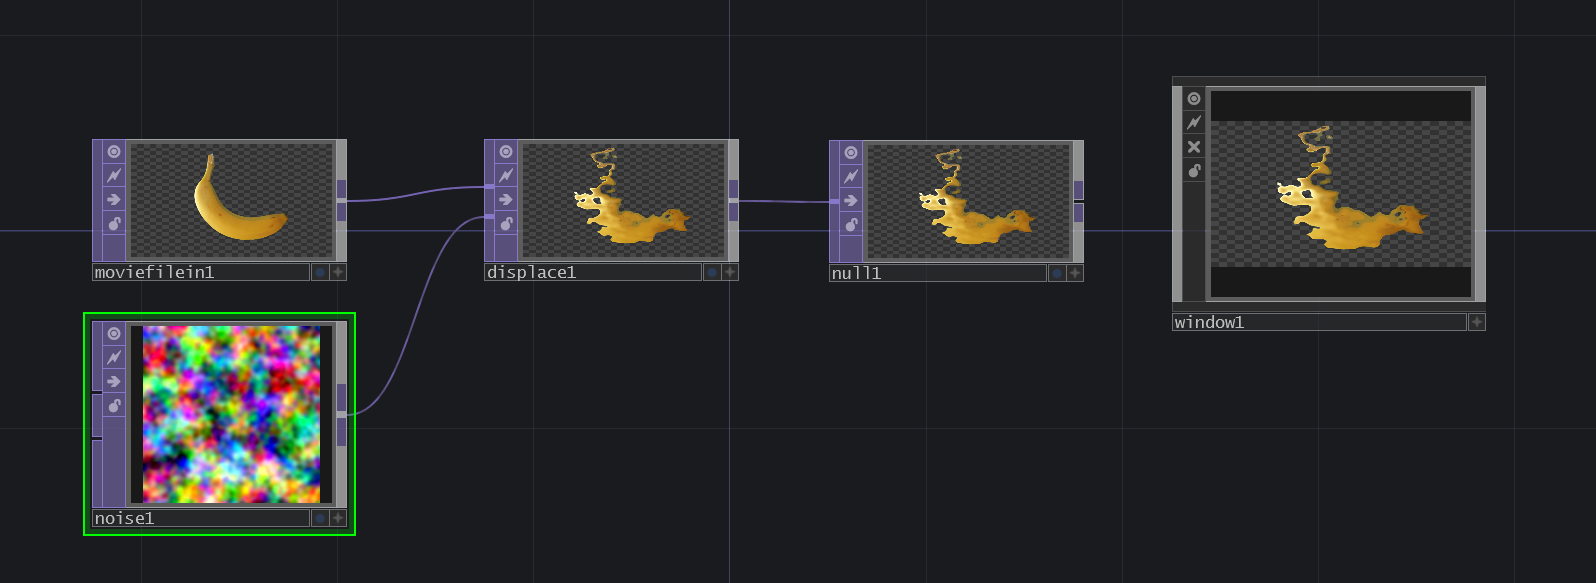
\includegraphics[width=\textwidth]{img/outputToWindow.PNG}
	\caption[shortCaption]
	{CAPTION MISSING}
	\label{fig:label}
\end{figure}




\begin{figure}[H]
	\centering
	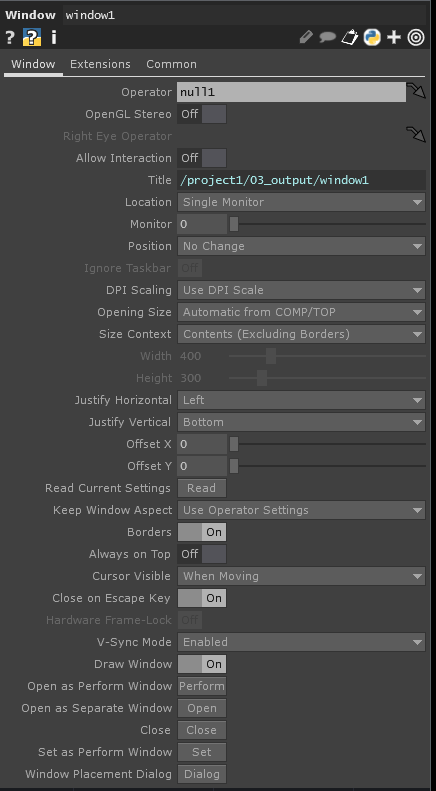
\includegraphics[width=8cm]{img/windowCompPars.PNG}
	\caption[shortCaption]
	{CAPTION MISSING}
	\label{fig:label}
\end{figure}


\section{CHOPs Introduction}
\begin{itemize}
\item Audio Device In \CHOP
\item Audio Device Out \CHOP
\item Audio File In \CHOP
\item Audio Filter \CHOP
\item Analysis \CHOP
\end{itemize}

\subsection{CHOP exporting}
\index{CHOP Exporting}


\subsection{Audio Analysis}
\index{Audio Analysis}

If we want to control the appearance of something, be it geometry/visuals or dmx/lights by an audio signal, we generally use the structure depicted in Figure \ref{fig:audioAnalysis2}.


	\begin{figure}[H]
	\centering


	\begin{tikzpicture}[auto, thick, node distance=2.3cm, >=triangle 45]

	\draw node at (5,0) [block] (audio) {\Large$Audio $};
	\draw node [block, right of=audio, node distance = 4cm] (fe) {\Large$Feature\ Extraction$};

	\draw node [block, right of=fe, node distance = 4cm] (mapping) {\Large$Mapping$};

	\draw node [block, right of=mapping, node distance = 3cm] (output) {\Large$Control$};

  \draw[->] (audio) -- node {}(fe);
  \draw[->] (fe) -- node {}(mapping);
  \draw[->] (mapping) -- node {}(output);

  \end{tikzpicture}
  \caption{Using Audio to control visual parameters.}
  \label{fig:audioAnalysis2}
\end{figure}


Audio digital signals are numbers. For a stereo signal, we get always 2 number in any moment of time. Also we typically get 44100 numbers per second per channel. So we get a lot of numbers, be it from a microphone, a sound card input or a file. \\
These numbers themselves are not directly suitable to control something video related.
Let's say we ignored on channel, so we get 44100 numbers per second. Let's assume we take these numbers to control the brightness of some video. First of all we will miss most of the action since our screens produce only 60 images per second if we are lucky. So we miss most of the 44100 values per second. And if we have really bad luck, these 60 images are all produced when the audio wave is passing through 0 or negative (audio signals typically move between -1 and 1). So our audio input could be really loud and our output could stay dark.\\

So we need some idea \textbf{what} we want to visualize. Loudness? The loudness of the bassdrum? The whole spectrum? We could think of many things and we will need some way to measure these. This process of measuring something about the audio is called \textit{Feature Extraction}. For a simple measure of loudness we could use the \textit{RMS}.\\

The next step might be to map this extracted measurement to a parameter, let's say the sized of a sphere. The linear RMS will range between 0 and 1. Now if we don't want the sphere to be 0 when the audio is silent, we will need to apply a \textit{mapping}. This just means that we take our RMS and by multiplication and addition, bring it in another range, for example we could add 1. Then our sphere will have a size of 1 in case of silence and double the size in case of maximal input RMS. In TouchDesigner, the Math \CHOP helps us a lot with this process. On its second page it offers us to map one range to another. We just have to tell it our input and output range and it does the remapping.\\
Beware that we could also apply a non-linear mapping, for example squaring or thresholding. We could look if the input is higher than some particular value and only then doe a certain action.




\subsection{Simple Spectrum Display}
\begin{figure}[H]
	\centering
	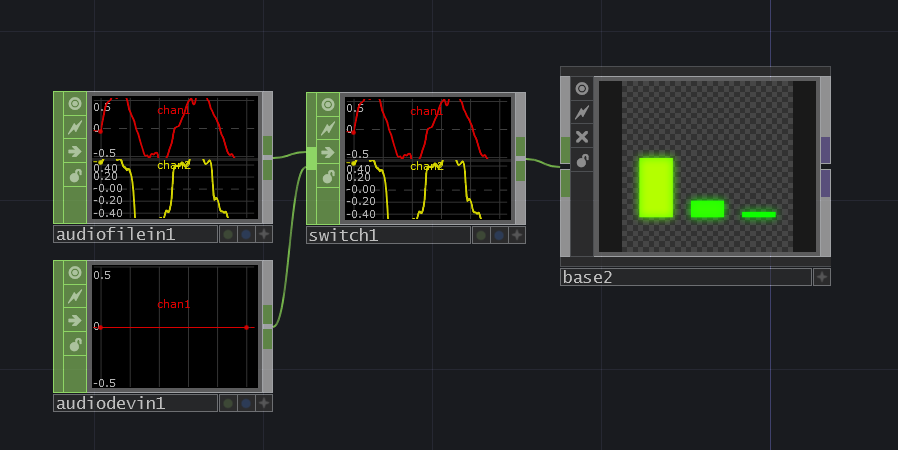
\includegraphics[width=\textwidth]{img/simpleSpecOverview.PNG}
	\caption[shortCaption]
	{CAPTION MISSING}
	\label{fig:label}
\end{figure}

\begin{figure}[H]
	\centering
	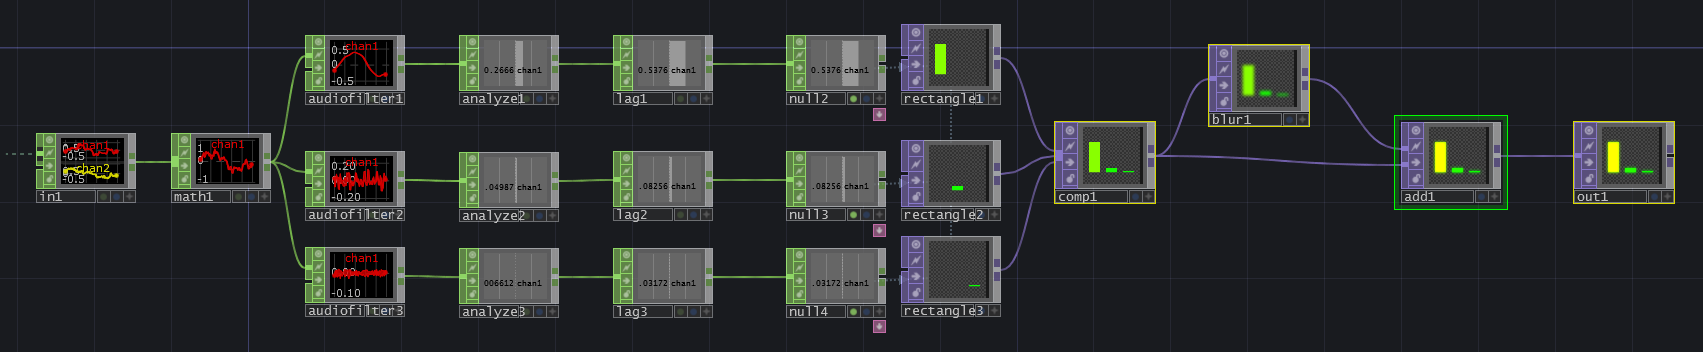
\includegraphics[width=\textwidth]{img/simpleSpec_inside.PNG}
	\caption[shortCaption]
	{CAPTION MISSING}
	\label{fig:label}
\end{figure}

